\documentclass[authoryear, 11pt, oneside]{report}

\pagestyle{headings} 
\usepackage{geometry} \geometry{a4paper} 
\usepackage[parfill]{parskip} 
\usepackage{natbib} 
\usepackage{graphicx} 
\usepackage{amssymb} 
\usepackage{epstopdf} 
\usepackage{rotating} 
\usepackage{setspace}
\usepackage{lscape}  \DeclareGraphicsRule{.tif}{png}{.png}{`convert #1 `dirname #1`/`basename #1 .tif`.png}
\usepackage{color}
\usepackage[pdftex,bookmarks,plainpages=false]{hyperref}
\usepackage{caption}
\usepackage{subcaption}
\usepackage{framed}

\usepackage{minted}
\usemintedstyle{trac}%perldoc}


\newcommand{\HRule}[1]{\hfill \rule{0.2\linewidth}{#1}} % Horizontal rule at the bottom of the page, adjust width here

\definecolor{grey}{rgb}{0.9,0.9,0.9} % Color of the box surrounding the title - these values can be changed to give the box a different color

\begin{document}



\thispagestyle{empty} % Remove page numbering on this page

%----------------------------------------------------------------------------------------
%	TITLE SECTION
%----------------------------------------------------------------------------------------

\colorbox{grey}{
	\parbox[t]{1.0\linewidth}{
		\centering \fontsize{150pt}{50pt}\selectfont % The first argument for fontsize is the font size of the text and the second is the line spacing - you may need to play with these for your particular title
		\vspace*{0.5cm} % Space between the start of the title and the top of the grey box
		
		\hfill  \\
		\centering How to run tools for Remote Sensing and GIS data processing using Docker and Singularity?\\
		\hfill  \\
		
		\vspace*{0.5cm} % Space between the end of the title and the bottom of the grey box
	}
}

\begin{center}
	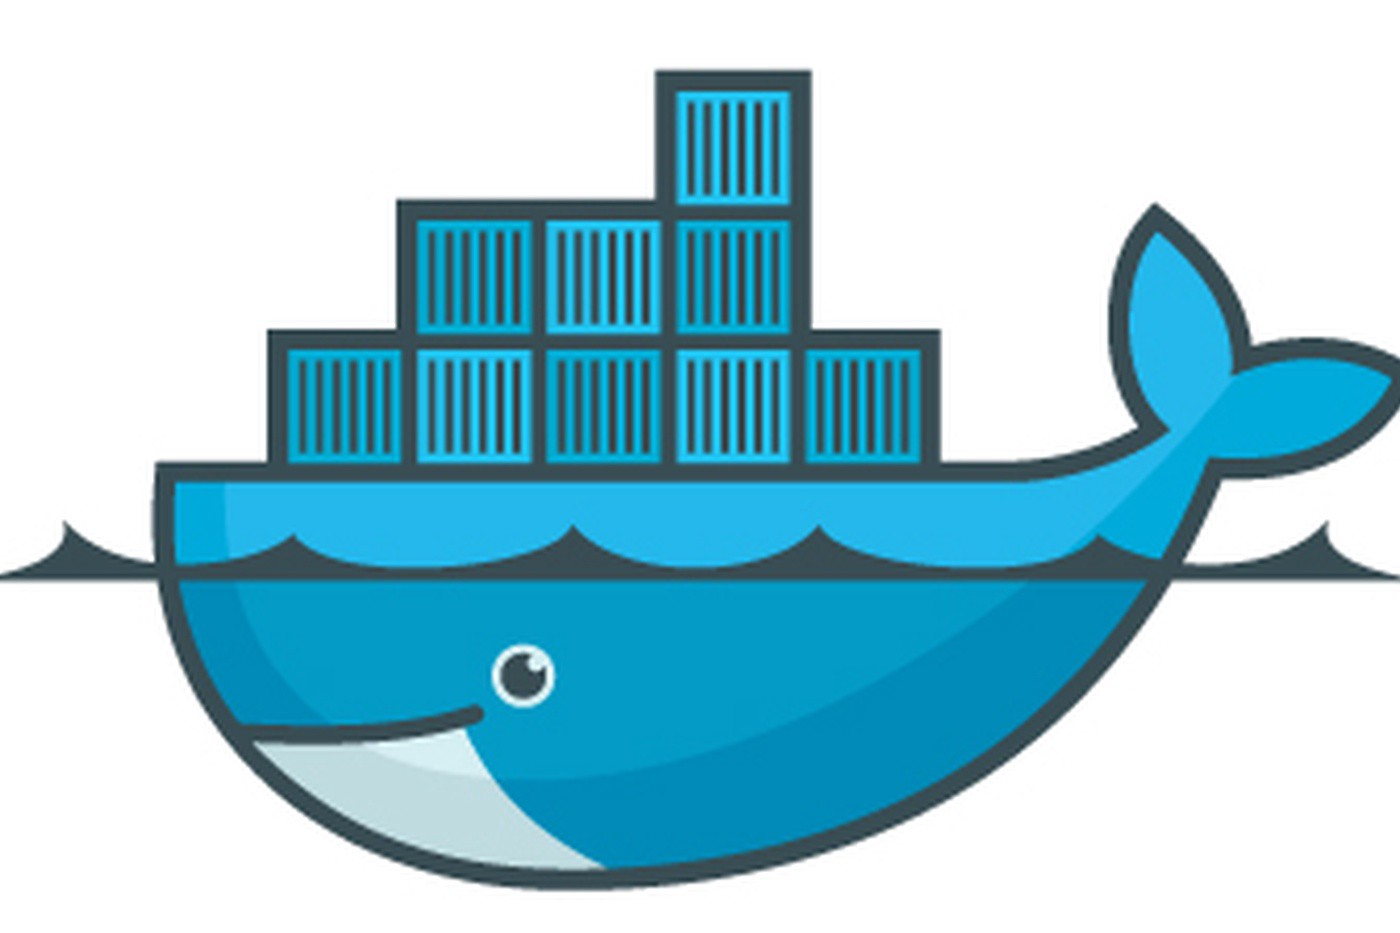
\includegraphics[width=0.55\columnwidth]{./figures/docker.jpeg}
	
\includegraphics[width=0.4\columnwidth]{./figures/s-logo.png}
\end{center}


%----------------------------------------------------------------------------------------

\vfill % Space between the title box and author information

%----------------------------------------------------------------------------------------
%	AUTHOR NAME AND INFORMATION SECTION
%----------------------------------------------------------------------------------------

{\centering \large 
\hfill Pete Bunting \\
\hfill Aberystwyth University \\
\hfill Earth Observation and Ecosystem Dynamics Group \\
\hfill Department of Geography and Earth Sciences \\
\hfill \url{pfb@aber.ac.uk} \\

\HRule{1pt}} % Horizontal line, thickness changed here

%----------------------------------------------------------------------------------------

\begin{center}
	
\includegraphics[width=\columnwidth]{./figures/Logos.pdf}
\end{center}

\clearpage % Whitespace to the end of the page




%\maketitle

\begin{framed}
This work (including scripts) is licensed under a Creative Commons Attribution 4.0 International License. To view a copy of this license, visit \url{http://creativecommons.org/licenses/by/4.0/}. 
\end{framed}

\begin{framed}
This document is focus on Docker containers which have been created by the Earth Observation and Ecosystem Dynamics (EOED) research group (\url{https://www.aber.ac.uk/en/dges/research/earth-observation-laboratory/}) at Aberystwyth University (\url{https://www.aber.ac.uk}) to support our research. These containers are focused on the tools and software we use for our data analysis and therefore do not include all possible relevant tools but feel free to use the Dockerfile's as a basis to create your own containers.
\end{framed}

\tableofcontents

\chapter{Containers}

\section{Why Containers?}

The two main software for container are Docker (\url{https://www.docker.com}) and Singularity (\url{https://sylabs.io}). Docker it more widely used and is available for Linux, MacOS and Windows, however it needs to run as a root user. While singularity can be executed without root privileges but is only available for Linux systems (although a beta version is available for MacOS).

Docker (\url{https://www.docker.com}) is a lightweight container system which creates a stand-alone executable package including everything needed to run the package: code, runtime, system tools, system libraries, settings.

A single container can can then be executed on multiple platforms without making any changes to the software or having to re-build the software. The container can also be tagged to create a unique version of the system encapsulated within the container which can be reused at a later point ensuring that a result can be reproduced.

In this case, whether the software is a built via spack (\url{https://spack.readthedocs.io}) or conda-forge (\url{https://conda-forge.org}) we can encapsulate the tools and dependencies within a docker container for re-use. 

\section{Where can Docker not be used?}

Docker cannot be used on a shared system (e.g., HPC) as it requires root access to execute which is not always possible or desirable. However, an alternative is available, which can import Docker containers, called Singularity (\url{https://sylabs.io/singularity/}) and this specifically supports HPC systems.

\section{Installing Docker}

\subsection{MacOS and Windows}

To install Docker, login into \url{https://hub.docker.com} and follow the instructions to download and install the software.

\subsection{Linux}

\subsubsection{Ubuntu / Debian}
 Instructions are available from \url{https://docs.docker.com/install/linux/docker-ce/ubuntu/} but if you have not previously had Docker installed then the following commands are used:
 
\begin{minted}[frame=lines]{bash}
sudo apt-get update
sudo apt-get install docker-ce docker-ce-cli containerd.io
\end{minted}

\subsubsection{CentOS}
 Instructions are available from \url{https://docs.docker.com/install/linux/docker-ce/centos/} but if you have not previously had Docker installed then the following commands are used:
 
\begin{minted}[frame=lines]{bash}
sudo yum install docker-ce docker-ce-cli containerd.io
\end{minted}

\subsubsection{Fedora}
 Instructions are available from \url{https://docs.docker.com/install/linux/docker-ce/fedora/} but if you have not previously had Docker installed then the following commands are used:
 
\begin{minted}[frame=lines]{bash}
sudo dnf install docker-ce docker-ce-cli containerd.io
\end{minted}

\section{Installing Singularity}

\subsection{Ubuntu}
\begin{minted}[frame=lines]{bash}
sudo apt-get install singularity-container
\end{minted}

\subsection{HPC}
If you are using a HPC system, such as Super Computing Wales (SCW) then singularity will need to be installed centrally, most likely via modules (\url{http://modules.sourceforge.net}) so you can loads singularity into your environment using a command such as:

\begin{minted}[frame=lines]{bash}
module load singularity
\end{minted}

\section{Useful Images/Containers}

NOTE Terminology: Docker has images and containers. A Docker Image is a set of files which have no state, whereas Docker Container is the instantiation of Docker Image. In other words, Docker Container is the run time instance of images.

On \url{https://hub.docker.com} you will find many useful Docker images which have been built and a ready to use.

The Docker images we will be using for the remainder of this tutorial are from myself and can be browsed at: \url{https://hub.docker.com/u/petebunting}.

\subsection{au-eoed}

This image contains the released version of RSGISLib (\url{https://www.rsgislib.org}) and ARCSI (\url{https://arcsi.remotesensing.info}) and their dependencies, such as GDAL (\url{https://gdal.org}). 

This is the image which most will want to use for satellite imagery analysis.

\subsubsection{URL}
\url{https://hub.docker.com/r/petebunting/au-eoed}

\subsubsection{Installation}

\begin{minted}[frame=lines]{bash}
docker pull petebunting/au-eoed
singularity pull docker://petebunting/au-eoed
\end{minted}

\subsection{spdlib}

This image contains the released version of SPDLib (\url{https://spdlib}) its dependencies, such as GDAL (\url{https://gdal.org}). 

This is the image which most will want to use for LiDAR data analysis.

\subsubsection{URL}
\url{https://hub.docker.com/r/petebunting/spdlib}

\subsubsection{Installation}

\begin{minted}[frame=lines]{bash}
docker pull petebunting/spdlib
singularity pull docker://petebunting/spdlib
\end{minted}


\subsection{au-eoed-micmac}

This image contains the released version of MicMac (\url{https://micmac.ensg.eu/index.php/Accueil}) its dependencies and scripts developed by the AU-EOED research group (\url{https://github.com/Ciaran1981/Sfm}) will allow processing of drone photogrammetry data. 

This is the image which most will want to use for processing drone photogrammetry data.

\subsubsection{URL}
\url{https://hub.docker.com/r/petebunting/au-eoed-micmac}

\subsubsection{Installation}

\begin{minted}[frame=lines]{bash}
docker pull petebunting/au-eoed-micmac
singularity pull docker://petebunting/au-eoed-micmac
\end{minted}


\subsection{au-eoed-dev}

This image contains the development version of RSGISLib (\url{https://www.rsgislib.org}), ARCSI (\url{https://arcsi.remotesensing.info}) EODataDown and other software create by the AU-EOED group and their dependencies, such as GDAL (\url{https://gdal.org}). 

This is the image should not be used in most cases as it changes regularly and at times may contain version of the software which are broken. However, it does contain the very latest versions of the various software and dependencies.

\subsubsection{URL}
\url{https://hub.docker.com/r/petebunting/au-eoed-dev}

\subsubsection{Installation}

\begin{minted}[frame=lines]{bash}
docker pull petebunting/au-eoed-dev
singularity pull docker://petebunting/au-eoed-dev
\end{minted}


\chapter{Docker: Running Data Analysis}

\section{Docker Tools}
Once you have pulled your Docker image it is installed on your system, to see which images you have downloaded to your system using the following command: 

\begin{minted}[frame=lines]{bash}
docker image ls
\end{minted}

To see which containers you have running you can use the following command:

\begin{minted}[frame=lines]{bash}
docker ps
\end{minted}

If you find that Docker is using a lot of storage space on your machine then the following command can be used to delete an image from your system:

\begin{minted}[frame=lines]{bash}
docker rmi <IMAGE ID>
\end{minted}

If you want to remove all components of the docker images/containers/volumes from your system then you can use the following command:

\begin{minted}[frame=lines]{bash}
# Remove any images or containers which are 'dangling'
docker system prune
# Remove any images or containers which are 'dangling' or stopped.
docker system prune -a
\end{minted}

\section{Container Terminal}

The simplest way to use the Docker image us to log into the container on a Terminal prompt. At this point your will have access to the software installed within the Docker image as you would from the Terminal on your own local machine. Running the following command will achieve this (NOTE: type \mintinline{bash}{exit} to leave the container):

\begin{minted}[frame=lines]{bash}
docker run -i -t petebunting/au-eoed /bin/bash
\end{minted}

Once within the container try and run a command such as \mintinline{bash}{gdalinfo --formats} to check the system is working.

However, you will noticed that you do not have access to your files, to get access to your local file system you need to mount this within the Docker container, as show below. NOTE: the variable \mintinline{bash}{${PWD}} is a reference to the current location (i.e., where in your file system you have run the docker image from) this is being mapped on to the \mintinline{bash}{/data} directory within the Docker container.

\begin{minted}[frame=lines]{bash}
docker run -i -t -v ${PWD}:/data petebunting/au-eoed /bin/bash
\end{minted}

From the terminal prompt within the Docker container you can now navigate to the \mintinline{bash}{/data} directory, if you list the contents of the directory you will find the same files as where you execute the \mintinline{bash}{docker run} command.

\begin{minted}[frame=lines]{bash}
cd /data
ls -lh
\end{minted}

You can also specify a specify local path to be mapped, for example:

\begin{minted}[frame=lines]{bash}
docker run -i -t -v /scratch/MyCoolData:/data petebunting/au-eoed /bin/bash
\end{minted}

Please note that you will now have to reference all your paths to \mintinline{bash}{/data} and not the local paths on the machine you are working from. Also, all the data and scripts you want to use also need to be available in \mintinline{bash}{/data}.

\section{ARCSI}

To run ARCSI using the docker image you use the same command as you would have otherwise done but you need to pre-append the Docker command and remember that all the files you are using are relative to the mount point within the Docker container.

\begin{minted}[frame=lines]{bash}
docker run -i -t -v /scratch:/data petebunting/au-eoed arcsi.py -s ls5tm\
-p CLOUDS DOSAOTSGL STDSREF SATURATE TOPOSHADOW FOOTPRINT METADATA \
-o /data/Outputs/ --tmpath /data/tmp --dem /data/UKSRTM_90m.kea \
--k  clouds.kea meta.json sat.kea toposhad.kea valid.kea stdsref.kea \
--stats --format KEA \
-i /data/Input/LT05_L1TP_203024_19950815_20180217_01_T1_MTL.txt
\end{minted}

\begin{minted}[frame=lines]{bash}
docker run -i -t -v /scratch:/data petebunting/au-eoed arcsi.py -s sen2 \
-p CLOUDS DOSAOTSGL STDSREF SATURATE TOPOSHADOW FOOTPRINT METADATA SHARP \
-o /data/Outputs  --dem /data/UKSRTM_90m.kea --tmpath /data/tmp \
--k  clouds.kea meta.json sat.kea toposhad.kea valid.kea stdsref.kea \
--stats --format KEA \
-i /data/S2A_MSIL1C_20170617T113321_N0205_R080_T30UVD.SAFE/MTD_MSIL1C.xml
\end{minted}

\section{Using GDAL Tools}

Using one of the GDAL tools is similar to the ARCSI, in that the commands are all the same but you need to update file paths to be relative to the mount point in the Docker container. For example:

\begin{minted}[frame=lines]{bash}
docker run -i -t -v /scratch:/data petebunting/au-eoed gdal_translate \
-of GTIFF /data/input_img.kea /data/output_img.tif
\end{minted}

\section{Running Python (RSGISLib)}

Again, the change which is needed related to the file paths either being inputting into the python script. For example, the following python script (saved as \mintinline{bash}{calc_ndvi.py})

\begin{minted}[frame=lines, linenos]{python}
import rsgislib.imagecalc

img = '/data/landsat_img.kea'
out_img = '/data/landsat_ndvi.kea'
rsgislib.imagecalc.calcindices.calcNDVI(img, 3, 4, out_img)

\end{minted}

Can be executed using the following Docker command:

\begin{minted}[frame=lines]{bash}
docker run -i -t -v /scratch:/data petebunting/au-eoed \
python /data/calc_ndvi.py
\end{minted}


\chapter{Singularity: Running Data Analysis}

Singularity doesn't store images centrally but as files on your system. 

\begin{minted}[frame=lines]{bash}
-rwxr-xr-x 1 pete pete 753M  Sep 24 20:15 au-eoed-20190327.simg
-rwxr-xr-x 1 pete pete 1000M Sep 24 17:02 au-eoed-dev-20190921.simg
\end{minted}

You can remove images by just deleting the files of the images you do no longer wish have on your system. I would recommend including the tag name (e.g., 20190921) in your singularity image name -- you might need to rename the file once it has downloaded. You choose the image to run by using the full path to the image file.

\section{ARCSI}

To run ARCSI using the singularity image you use the same command as you would have otherwise done but you need to pre-append the Singularity command.

\begin{minted}[frame=lines]{bash}
singularity exec /data/sw_imgs/au-eoed-20190327.simg arcsi.py -s ls5tm\
-p CLOUDS DOSAOTSGL STDSREF SATURATE TOPOSHADOW FOOTPRINT METADATA \
-o ./Outputs/ --tmpath ./tmp --dem ./UKSRTM_90m.kea \
--k  clouds.kea meta.json sat.kea toposhad.kea valid.kea stdsref.kea \
--stats --format KEA \
-i ./Input/LT05_L1TP_203024_19950815_20180217_01_T1_MTL.txt
\end{minted}
\newpage
\begin{minted}[frame=lines]{bash}
singularity exec /data/sw_imgs/au-eoed-20190327.simg arcsi.py -s sen2 \
-p CLOUDS DOSAOTSGL STDSREF SATURATE TOPOSHADOW FOOTPRINT METADATA SHARP \
-o ./Outputs  --dem ./UKSRTM_90m.kea --tmpath ./tmp \
--k  clouds.kea meta.json sat.kea toposhad.kea valid.kea stdsref.kea \
--stats --format KEA \
-i ./S2A_MSIL1C_20170617T113321_N0205_R080_T30UVD.SAFE/MTD_MSIL1C.xml
\end{minted}

\section{Using GDAL Tools}

Using one of the GDAL tools is similar to the ARCSI, in that the commands are all the same, but you need pre-append the singularity command and image file. For example:

\begin{minted}[frame=lines]{bash}
singularity exec /data/sw_imgs/au-eoed-20190327.simg gdal_translate \
-of GTIFF ./input_img.kea ./output_img.tif
\end{minted}

\section{Running Python (RSGISLib)}

Again, the change which is needed related to the file paths either being inputting into the python script. For example, the following python script (saved as \mintinline{bash}{calc_ndvi.py})

\begin{minted}[frame=lines, linenos]{python}
import rsgislib.imagecalc

img = '/scratch/a.pfb/landsat_img.kea'
out_img = '/scratch/a.pfb/landsat_ndvi.kea'
rsgislib.imagecalc.calcindices.calcNDVI(img, 3, 4, out_img)

\end{minted}

Can be executed using the following Singularity command:

\begin{minted}[frame=lines]{bash}
singularity exec /data/sw_imgs/au-eoed-20190327.simg \
python /data/calc_ndvi.py
\end{minted}

\chapter{Batch Processing Landsat with Docker and ARCSI}

ARCSI has tools for bulk downloading and processing landsat and sentinel-2 data but require the Google Cloud SDK, the following commands can be used with two different docker images (\mintinline{bash}{petebunting/au-eoed-dev} and \mintinline{bash}{google/cloud-sdk})

\section{Download Landsat Database}
The following command will download and build a local sqlite database for all the Landsat images collected globally:
\begin{minted}[frame=lines]{bash}
docker run -i -t -v ${PWD}:/data petebunting/au-eoed-dev \
arcsisetuplandsatdb.py -f /data/lsgoog_db_20190924.sqlite
\end{minted}

\section{Search Landsat for Scenes}
The following command searches the local database for path 227 and row 63 for collection 1 scenes and a cloud cover less than 50 percent.
\begin{minted}[frame=lines]{bash}
docker run -i -t -v ${PWD}:/data petebunting/au-eoed-dev \
arcsigenlandsatdownlst.py -f /data/lsgoog_db_20190924.sqlite \
-p 227 -r 63 -o /data/ls_scns_dwnld.sh --outpath /data/ls_dwn \
--collection T1 --cloudcover 50 --multi --lstcmds
\end{minted}

\section{Setup Google SDK}
If this is the first time you are using this google cloud sdk docker image, then you will need to authenticate it using the following command:
\begin{minted}[frame=lines]{bash}
docker run -ti --name gcloud-config google/cloud-sdk gcloud auth login
\end{minted}

\section{Download Landsat Images}
To download the scenes which were found through querying the database and outputted into file \mintinline{bash}{/data/ls_scns_dwnld.sh} the following command: 
\begin{minted}[frame=lines]{bash}
docker run -ti -e CLOUDSDK_CONFIG=/config/mygcloud \
-v ${PWD}/mygcloud:/config/mygcloud -v ${PWD}:/certs \
-v ${PWD}:/data  google/cloud-sdk sh /data/ls_scns_dwnld.sh
\end{minted}

\section{Generate ARCSI Commands}
The following command can be used to generate ARCSI commands for processing all the scenes which have been downloaded:
\begin{minted}[frame=lines]{bash}
docker run -i -t -v ${PWD}:/data petebunting/au-eoed-dev 
arcsibuildcmdslist.py -s LANDSAT -f KEA --stats \
-p CLOUDS DOSAOTSGL STDSREF --outpath /data/ls_ard \
--dem /data/srtm/srtm_3arc.kea --tmpath /data/tmp \
--keepfileends stdsref.kea clouds.kea -i /data/ls_dwn 
-e "*MTL.txt" -o /data/ard_arcsi_cmds.sh
\end{minted}

\section{Run ARCSI Commands with Docker}
The commands outputted do not have the docker command pre-appended so that needs to be pre-appended at the front of all the lines, so more cores can be used for the processing the following command can be used to split it into 4 output files:
\begin{minted}[frame=lines]{bash}
docker run -i -t -v ${PWD}:/data petebunting/au-eoed-dev \
splitcmdslist.py -i /data/ard_arcsi_cmds.sh \
-p "docker run -i -t -v ${PWD}:/data petebunting/au-eoed-dev" \
-o /data/ard_arcsi_cmds_splt.sh -f 4
\end{minted}

The output files can then be execute in different terminal windows using the following commands:
\begin{minted}[frame=lines]{bash}
sh ard_arcsi_cmds_splt_1.sh
sh ard_arcsi_cmds_splt_2.sh
sh ard_arcsi_cmds_splt_3.sh
sh ard_arcsi_cmds_splt_4.sh
\end{minted}

\chapter{Conclusion}

Docker and Singularity are a really useful set of tools and solve a lot of challenges with software installation and deployment and transferring workflows between different machines (e.g., local laptop, workstation, HPC and Amazon or Google Cloud).

It is recommended that you develop your workflow and scripts on your local machine, probably using Docker, and then deploy onto the HPC or high performance workstation using Singularity.

\end{document}  
